\begin{figure}[ht]
\centering
	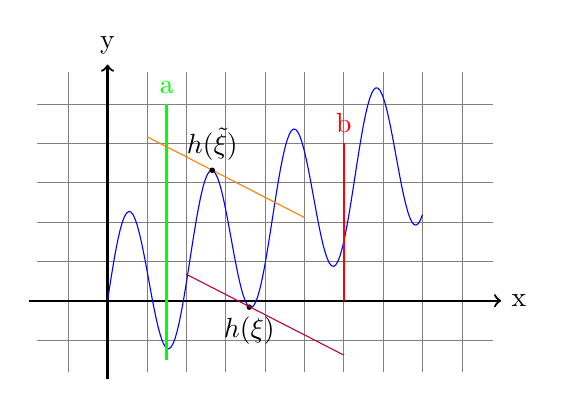
\begin{tikzpicture}
		\draw[very thin, gray, step = 0.5] (-0.9,-0.9) grid (4.9,2.9);
		\draw[->,thick, black](-1,0) -- (5,0) node[right]{x};
		\draw[->,thick, black](0,-1) -- (0,3) node[above]{y};
		\draw[blue,domain = 0.0:4.0, samples=150]   
			plot (\x,{(sin(6*\x r))+ 0.5*\x});
       	\draw[green,thick](0.75,-0.75)--(0.75,2.5)node[above]{a};
       	\draw[red,thick](3,0) -- (3,2) node[above]{b};
       	\draw[black](1.33,2.34079);
       	\draw[orange,domain = 0.5:2.5, samples = 150]
       		plot(\x,-0.5133*\x+2.3407);
       	\fill[black](1.33,1.657)circle(1pt)node[above]{$h(\tilde{\xi})$};
       	\fill[black](1.8,-0.0809)circle(1pt)node[below]{$h(\xi)$};
       	\draw[purple,domain = 1:3, samples = 150]
       		plot(\x,-0.5133*\x+0.85);
	\end{tikzpicture}
\end{figure}